\begin{figure}[htbp]
\begin{centering}
\resizebox{\columnwidth}{!}
{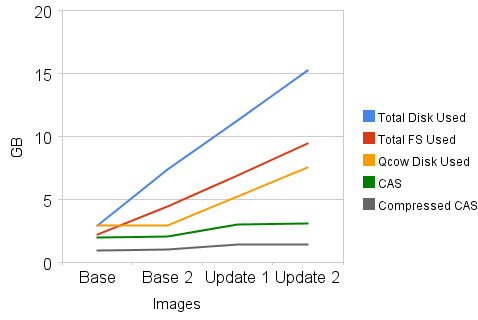
\includegraphics{venti_analysis}}
\small\itshape
\caption{\small\itshape Efficiency of Underlying Storage Technique}
\label{fig:venti}
\end{centering}
\end{figure}

Finally, to validate whether or not content addressable storage schemes
would improve storage efficiency in the face of software-updates we compared
the disk overhead of two instances of a Linux installation before and after
a software update.  We compared raw disk utilization, file system reported
space used, copy-on-write image disk utilization, content addressable storage,
and compressed content addressable storage.
To construct the copy-on-write images, we used the QEMU QCOW2 format and
used the same base image for both \emph{Base} and \emph{Base2}.
To evaluate the content addressable storage efficiency we used Venti to
snapshot the raw disk images after installation and again after a manual
software update was run.  We used Venti's web interface to collect data about
its storage utilization for compressed data as well as its projections for
uncompressed data.

As can be seen in Figure~\ref{fig:venti} the various solutions all take
approximately the same amount of storage for a single image.  When adding
a second instance of the same image, the raw storage use doubles while both
the copy-on-write storage and content-addressable-storage essentially remain
the same.
The software update process on each image downloaded approximately 500MB of 
data.  As the update applied, each QCOW2 image (as well as the raw disk
images) increased in size proportionally.

We were surprised to find both the raw disk and copy-on-write overhead for the
software update was over double what we expected.  
We surmise this is due to temporary files and other transient data written
to the disk and therefore the copy-on-write layer.
This same dirty-but-unused block data is also responsible for the 
divergence between the \emph{Total FS Used} and the \emph{Total Disk Used} 
lines in the reported storage utilization.
This behavior paints a very bad efficiency picture for copy-on-write 
solutions in the long term.
While copy-on-write provides some initial benefits, their storage utilization
will steadily increase and start to converge with the amount of
storage used by a raw-disk installation.

Utilizing the disk block scanning techniques we applied in Section 2, we
found we could detect and de-duplicated these transient dirty blocks.
Such an approach may work to improve overall performance once we work out
the scalability and performance issues of the underlying CAS mechanism.
Because Venti is partially aware of the underlying structure of the Ext2
file system it only snapshots active file blocks.  
As a result, its storage utilization grows slightly for the
first software update, but the overhead of the second software update is
completely eliminated. 

